% -*- root: ../SI2.tex -*-

  \begin{problem}[1]
  Diseñar, a nivel de bloques, un sistema por el cual un \textit{middleware} pudiera soportar redundancia en un servidor de archivos planos (tipo disco
  compartido) de modo transparente a la aplicación y los servidores
  que intervienen en la conexión.


  \solution



  \end{problem}

  \begin{problem}[2]
  Uno de los principales problemas que tiene que tratar cualquier
\textit{middleware} que comunique ordenadores de distinto tipo es la transparencia del formato
  de representación interno de los datos en cada componente de la
  red. Estudiar las ventajas e incovenientes de cada una de estas tres posibles
  alternativas en distintas situaciones de sistemas distribuidos:
    \begin{itemize}
    \item Convertir todos los datos al formato interno de uno de los componentes
    de la red.
    \item Convertir todos los datos a un formato intermedio de intercambio.
    \item No realizar ninguna conversión en el \textit{Middleware}, y dejar que cada
aplicación realice las conversiones que considere oportunas.
\end{itemize}
    \solution
\textcolor{green}{Dejuan opina que:}

Convertir todos los datos a un formato intermedio requiere que tanto el cliente como el servidor realicen una conversión. Si pensamos en términos de idiomas entre personas se entiende muy fácilmente. Si yo hablo ruso y tu chino, ¿para qué vamos a aprender los 2 español?

Mejor será que yo aprenda chino o tu ruso, es decir, convertir todos los datos al formato de uno de los componentes require menos trabajo (por lo menos a los componentes que no tienen que convertir nada).

En cuanto a no realizar ninguna conversión, la ventaja que presenta es que el middleware es un software más ligero porque tiene menos funciones, pero presenta la gran desventaja de que a los desarrolladores les obliga a conocer las representaciones internas de los datos de los componentes del sistema distribuido y les añade una complejidad innecesaria.

    \end{problem}

  \begin{problem}[3]
  En un sistema de comunicaciones mediante RPCs, estudiar el lugar adecuado
para introducir la función de conversión del formato de representación de los
datos descrita en el problema anterior. Nota: Basarse en la figura \ref{RPCimg}.
  \solution

\textcolor{green}{Dejuan opina que:}

Suponiendo que el formato elegido sea el del servidor, el cliente tendría que realizar el \textit{marshalling} al enviar un RPC en el momentos 2 (al enviar) y el \textit{unmarshalling} en el 10 (al recibir) de la imagen, cuando el \textit{Client stub} codifica y descodifica\footnote{tal vez codifica y descodifica no son las palabras adecuadas} respectivamente el mensaje para dárselo al nivel de transporte.

  \end{problem}

  \begin{problem}[4]
  Sugerir alguna alternativa al servicio \textit{portmapper} empleado en la
comunicación mediante RPCs para conocer la dirección (puerto) del servidor
con el que se desea comunicar, basado en alguno de los servicios que puede
desempeñar un \textit{middleware}.
  \solution

\textcolor{green}{Dejuan opina que:}


RM-ODP define que el NOS \ref{NOS} (una de las 3 capas del middleware) puede proporcionar transparencia ofreciendo un servicio de nombres y transparencia a la ubicación, movilidad y reubicación.

Si se definiera un espacio de nombres o se incluyera la funcionalidad de conocer los puertos en el NOS solucionaríamos la necesidad del \textit{portmapper}

  \end{problem}

  \begin{problem}[5]
  Un determinado sistema distribuido requiere que cada servidor autentique
  la conexión de sus clientes mediante la introducción de un
  identificador de usuario y una contraseña. Supuesto que posee un
  \textit{middleware} genérico, diseñar sobre él un servicio que permita a las
aplicaciones clientes realizar una validación única de usuario y contraseña,
independientemente del número de servicios que sea necesario utilizar.
  \solution

\textcolor{green}{Dejuan opina que:}


No entiendo bien la pregunta. Para diseñarlo en serio haría falta más información.

Por middleware genérico tampoco entiendo qué incluye. Una de las características deseables del NOS es \textit{Single Sign On, SSO}, un único usuario y contraseña para todos los servicios. Si el middleware genérico que tenemos incluye un NOS con SSO, entonces tendríamos que añadir la funcionalidad de permitir inicio de sesión distribuido, sabiendo que el usuario y la contraseña es la misma para todo el sistema.

\yoP

Entiendo que lo que piden es describir una arquitectura o procedimiento que te permita llevar a cabo esta tarea.

Suponiendo que tenemos un sistema con varios servidores, podemos hacer que uno de ellos sea el encargado de la autenticación de los usuarios. Una vez que este servidor comprueba que tienes permisos de acceso te devuelve un identificador y el mismo identificador codificado con su clave privada (a modo de firma).

Cada vez que el cliente conecte con alguno de los servidores, enviará este identificador junto con la firma con lo que el servidor destino sólo tendrá que coger su clave para comprobar que el cliente ya está loggeado.

Al margen de las claves que permitan relacionarse a un servidor con otro a través del cliente de modo seguro, serían necesarias más pares de claves de modo que la comunicación cliente-servidor también fuese segura.
  \end{problem}

  \begin{problem}[6]
  Partiendo del esquema de comunicación entre programas a través de la
interfaz \textit{socket} (\ref{SocketNoConexion}), ampliar el esquema correspondiente al programa servidor para que sea capaz de atender conexiones simultáneas de varios programas clientes.

Sugerencia: Utilizar una tarea en el servidor por cada conexión.
  \solution

\textcolor{green}{Dejuan opina que:}

La interfaz de socket a la que se refiere el enunciado (la de la página 12 de las transparencias) es socket no orientado a conexión.

Para poder atender simultáneamente conexiones, habría que crear hilos antes del \textit{rcvfrom()} para que atendieran a los diversos clientes.


  \end{problem}

  \begin{problem}[7]
  Un sistema de control de inventario central recibe los movimientos de
mercancía que se realizan en su red de almacenes, y de ellos debe ser capaz en
todo momento de conocer la cantidad de cada producto que existe en toda la red.
Proponer el mecanismo de comunicaciones que se considere más adecuado para
realizar estos envíos, considerando distintos casos:

    \ppart Todos los sistemas operan simultáneamente, y disponen de enlaces de
comunicaciones dedicados.
    \ppart Todos los sistemas operan simultáneamente, pero los enlaces de que disponen
son conmutados.
    \ppart Los sistemas tienen distinto horario de funcionamiento.

    \solution

    \yoP

    Entendemos que tenemos un sistema de varios servidores (conectados, obviamente, a muchos clientes pero eso no nos importa) y queremos que estén correctamente sincronizados estos servidores, de modo que si un cliente compra algo, el stock de todos se reduzca.

    \spart

    Si tienen enlaces de comunicación dedicados es posible que cada servidor informe al resto en tiempo real de todos los cambios que se experimentan, de modo que todos los servidores pudieran tener siempre información actualizada.

    \spart
    Si los enlaces son conmutados, al mandar un servidor un mensaje, el enlace queda bloqueado, por lo que una comunicación en tiempo real no sería viable. \textcolor{blue}{No se exactamente qué se debería hacer aquí}

    \spart

    Por definición, parece que lo óptimo es el empleo de una cola de mensajes donde los servidores informan de los cambios. Cuando un servidor arranque, antes de empezar a trabajar, actualiza su información en base a los mensajes de la cola.

    \end{problem}

  \begin{problem}[8]
  Nombrar casos de comunicación entre aplicaciones en los que sea
preferible emplear colas no persistentes en lugar de colas persistentes.
Razonar la respuesta.
  \solution

\textcolor{green}{Dejuan opina que:}

Recordamos que persistencia en colas significa que persistan los mensajes de la cola, no la cola en sí. (La persistencia de la cola se llama temporalidad).

Si eres el de misión imposible y quieres que los mensajes con la misión que mandas se autodestruyan, puede ser interesante implementar una cola no persistente.

\yoP

En general puede ser interesante cuando no te preocupe preservar o no los mensajes, puesto que hacer la cola persistente implica un coste extra que puedes ahorrar.

No creo que haya ningún momento en que te interese perder la información, simplemente puede darse el caso de que no rente el coste necesario para mantener esos mensajes en caso de fallo.


  \end{problem}

  \begin{problem}[9]
  Enumerar las ventajas e inconvenientes que puede tener sustituir un mecanismo
  de comunicación entre procesos interno de un sistema operativo (áeras
  de memoria compartidas, archivos, \textit{named pipes}, etc.) por colas locales
de \textit{MQSeries} para comunicar dos aplicaciones en el mismo ordenador.
Justificar brevemente cada una de ellas.
  \solution

  \yoP

  Para empezar es posible que no nos interese emplear colas de mensajes. Si necesitamos que una aplicación espere hasta que la otra finalice el proceso nos interesará emplear mecanismos de comunicación como los sockets en lugar de colas.

  Puestos a que nos interese el empleo de colas, las colas de MQSeries tienen el problema de que implican más carga de trabajo para el sistema operativo, pues en el fondo serán otro programa que se está ejecutando en el mismo host.

  Una posible ventaja del empleo de colas MQSeries es que, si tienen appis adecuadas para distintos lenguajes de programación, puede ser más sencilla la comunicación con ellas, pues las llamadas al sistema no son igual de sencillas en todos los lenguajes.

  Frente al empleo de áreas de memoria compartidas o sistemas de archivos, se tiene la ventaja de que las colas de mensajes, y en concreto las de MQSeries, permiten gestionar fácilmente el control de los mensajes leídos y los destinatarios de los mismos.


  \end{problem}

  \begin{problem}[10]
  Un sistema de directorio de nombres jerárquico consta de un nodo raíz, que
denominaremos A, y tres nodos secundarios que dependen de él, que denominaremos
B, C y D, respectivamente. No existe replicación de la información en ninguno
de los servidores de nombres de la estructura, de modo que cada servidor sólo
contiene la información de las estaciones que dependen de él. Expresar el flujo
de mensajes que debe tener lugar para que una estación del nodo B, que
denominaremos B1, pueda recuperar la información de directorio de una estación
dependiente del nodo C, denominada C1.
  \solution

  \yoP

  \begin{enumerate}
  \item[1] B1 pregunta a B por C1
  \item[2] B no conoce a C1 (sólo conoce a las estaciones que dependen de él), así que manda a B1 a preguntar a A, pasándole su dirección IP

  \item[3] B1 pregunta a A por C1 y A reconoce que estará asociado a C por que le envía a B1 la dirección de C. \textcolor{blue}{Dejuan opina que A debería preguntar a C y a D a ver de quién es C1, porque A sólo conoce los que dependen de Él, ¿no?}

  \textcolor{red}{Pedro manda a de Juan y a aquellos que tengan esta duda a mirar el ejercicio 20, que resolvió la profesora y en el que se observa que tu no buscas C1 a pelo sino que lo buscas conociendo su nombre completo. Es decir, estás buscando A.C.C1}

  \item[4] B1 pregunta a C por C1 y este, puesto que C1 depende de él, lo conoce y le dice a B1 la dirección de C1
  \item[5] B1 conecta con C1
  \end{enumerate}

  \end{problem}

  \begin{problem}[11]
  Determinar la tolerancia mínima de reloj que es necesario considerar
  debido a la propagación de la información por el medio físico en un sistema
  que sincronice desde un servidor de tiempo central los relojes de todas
  sus estaciones en los siguientes casos:
    \ppart Entorno de red de área local de un tamaño máximo de 500 m.
    \ppart Entorno de red de área extendida, máxima distancia de 600 Km.
    \ppart Entorno de red transoceánica por cable coaxial, máxima distancia entre
nodos de 10.000 Km.
    \ppart Red VSAT \textit{(Very Small Aperture Terminal}, red de comunicaciones vía
satélite) con nodo de retransmisión en un satélite en la órbita geoestacionaria
(36.000 Km. sobre el ecuador).
  \paragraph{Notas: }
  - Considerar la velocidad de propagación de un campo electromagnético
en un cable aproximadamente igual a 2/3 de la velocidad de la luz en el
vacío.

  - No se consideran efectos de elementos intermedios de la comunicación,
  ni a nivel físico (amplificadores,  regeneradores de señal) ni a niveles
  superiores (puentes o \textit{routers}).

  \solution

  \yoP

  Me niego a hacer los cálculos, hacemos cuentas para obtener el tiempo de transporte y atendiendo a las cuentas realizadas en el ejemplo \ref{ejemplo_tiempos}, vemos que la tolerancia mínima es $\pm\frac{t+t'}{2}$ donde $t$ y $t'$ son los tiempos de transporte del mensaje en ambas direcciones.

\textcolor{green}{Dejuan se anima a hacer las cuentas}

Recordamos que la velocidad de la luz es $c=3·10^8 m/s$, con lo que $v_p=2·10^8m/s$.

\spart
\[
t = \frac{d}{v_p} = \frac{500m}{2·10^8m/s} = 2.5·10^{-6}  s
\]
\spart
\[
t = \frac{d}{v_p} = \frac{600Km}{2·10^8m/s} = 3·10^{-3} s
\]
\spart
\[
t = \frac{d}{v_p} = \frac{10^6m}{2·10^8m/s} = 5·10^{-2} s
\]
\spart
\[
t = \frac{d}{v_p} = \frac{36·10^6m}{2·10^8} =  1.8·10^{-1} s
\]
  \end{problem}

  \begin{problem}[12] A efectos de asignación de nombres a los distintos recursos
  que lo componen, un determinado sistema distribuido se encuentra dividido
  en distintos dominios administrativos, organizados de modo jerárquico
  según al esquema:

  \begin{center}
  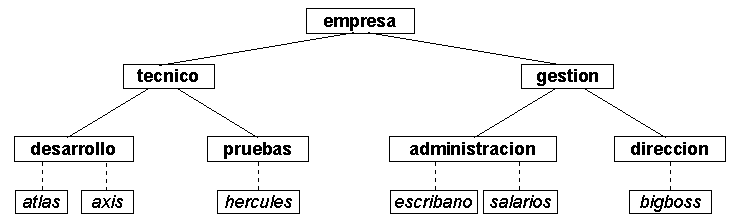
\includegraphics[width=1\textwidth]{img/si2-t4-ej-dom1.png}
  \label{Subnormalidad.}
  \end{center}

  Los nodos en cursiva representan ordenadores, y los nodos en negrita, los dominios.


  Cada dominio tiene un servidor de nombres propio, que reside en un ordenador
    cuyo nombre coincide con el del dominio, con capacidad de almacenamiento local
    de resultados de consultas a otros dominios (cache). Inicialmente se supone que
    todas las caches de los dominios se encuentran vacías.

    \ppart Poner los nombres completos en el dominio global de cada uno de los
      ordenadores representados en cursiva en la figura.
    \ppart Detallar los mensajes que serán necesarios y entre qué sistemas deben
        circular para que el ordenador atlas localice el servidor salarios en el
        directorio a partir de su nombre en la red.
      \ppart Inmediatamente después de la anterior consulta, el ordenador axis necesita
          establecer una conexión con salarios. Indicar el flujo de mensajes que ocurrirá
        para que pueda localizarlo en el directorio.
      \ppart Supuesto que el sistema de nombres que se emplea sigue el estándar X.500, nombrar:
            \begin{itemize}
              \item Ordenadores que contendrán un \textit{Directory User Agent}.
              \item Ordenadores que contendrán un \textit{Directory System Agent}.
              \item Tres parejas de ordenadores entre las que se empleará un \textit{Directory Access Protocol}.
              \item Tres parejas de ordenadores entre las que se empleará un \textit{Directory System Protocol}.
            \end{itemize}
      \ppart Proponer un sistema de comunicaciones (\textit{peer to peer} orientado a conexión, no orientado a conexión, \textit{Remote Procedure Calls},
 colas de mensajes) para producir los intercambios de mensajes de
resolución de nombres en el directorio, y razonar la respuesta.


\solution

\yoP

\spart

No pienso escribirlos todos. Es trivial. Por ejemplo, en el caso del host \textit{hércules} su nombre completo en el dominio global sería \textit{empresa/técnico/pruebas/hércules}

\spart

Equivalente al ejercicio 10.

\begin{enumerate}
\item[1] \textit{Atlas} pregunta a \textit{desarrollo} por \textit{salarios}
\item[2] \textit{Desarrollo} pregunta a \textit{técnico} por \textit{salarios}
\item[3] \textit{Técino} pregunta a \textit{empresa} por \textit{salarios}
\item[4] \textit{Empresa} pregunta a \textit{gestión} por \textit{salarios}
\item[5] \textit{Gestión} pregunta a \textit{administración} \textcolor{blue}{y a dirección (según Dejuan)} por \textit{salarios}
\item[6] \textit{Administración} envía a \textit{gestión} la dirección de \textit{salarios}
\item[7] El mensaje recorre la cadena en dirección contraria hasta llegar a \textit{atlas}
\end{enumerate}

\spart

Suponiendo que los servidores guardan en la caché información de las consultas recientes, el servidor \textit{desarrollo} ya tiene guardado en caché la dirección de \textit{salarios}, por lo que le responde directamente a \textit{axis}

\spart

\begin{itemize}
\item \textbf{Directory User Agent}:

Los que están en cursiva
\item \textbf{Directory System Agent}

Los que están en negrita
\item \textbf{Directory Acces Protocol}

\subitem axis-atlas
\subitem atlas-hércules
\subitem salarios-bigboss

\item \textbf{Directory System Protocol}
\subitem desarrollo-técinico
\subitem empresa-gestión
\subitem administración-dirección
\end{itemize}

\spart

La cola de mensajes no tiene sentido pues necesitamos obtener respuestas en tiempo real.

Peer to peer tampoco termina de encajar con la lógica del sistema, pues hay un claro comportamiento jerárquico y cada host pregunta de forma única a otro host y no pregunta a un tercero hasta no obtener su respuesta.

El método más interesante sería RPC donde cada host establece comunicación directa con aquel con el que quiere comunicarse. Además no tenemos que preocuparnos por la representación interna de los datos por lo que cada no podría estar programado en un lenguaje completamente diferente.

\textcolor{blue}{A Dejuan no le gusta RPC} porque no necesitamos ejecutar funciones que se encuentren en otros servidores, simplemente queremos hacer una pequeña consulta por lo que lo que más le convence es \textit{peer to peer} (porque no sólo hablas con el de arriba sino también con los que puedan tener debajo) y como no son muy frecuentes las consultas (debido a la caché) opina que lo ideal sería no orientado a conexión.

\end{problem}


  \begin{problem}[13]
  Se desea realizar un servidor para una red de área local que actúe como
punto focal de recepción de alarmas que se produzcan en las estaciones de
trabajo ante situaciones de diversos tipos (conexión de estación, fallos de
programas, errores en disco,introducciones de contraseñas equivocadas, etc.).

    \ppart Enumerar los mecanismos de comunicaciones que se pueden emplear para
enlazar los clientes con el servidor para realizar esta función u otras
similares.

    \ppart Valorar el empleo de cada uno de los mecanismos anteriores para realizar la
aplicación, y elegir la que se considere más apropiada a este caso, razonando
la respuesta.
    \ppart Si el prototipo de función que se desea utilizar en las estaciones clientes
para enviar una alerta es el siguiente:
\begin{verbnobox}[\small]
long alerta (
char tipo_alerta,      // Tipo de alerta que se ha producido
char nivel_gravedad,   // Nivel de gravedad de la misma
char * datos_adicionales,// Texto informativo dado por el cliente
long * codigo_accion   // Acción recomendada por el servidor
);                     //  para resolver la situación.
\end{verbnobox}
    en la que el valor que retorna la función indica si se ha completado
correctamente o no la función, tanto por motivos de la red como del servidor,
definir:
    \begin{itemize}
      \item Una estructura de mensaje apropiada para la comunicación entre cliente y
servidor.
      \item Explicar el proceso de \textit{Parameter Marshalling} que será necesario
realizar en el cliente antes del envío del mensaje. (Sugerencia: emplear C o
pseudocódigo, comentado).
      \item Explicar el proceso de \textit{Parameter Unmarshalling} que será necesario
realizar en el cliente al recibir el mensaje de contestación. (Igual sugerencia).
    \end{itemize}
      \solution

      \yoP

      \spart

      Puestos a enumerar tendríamos: WS, P2P, RPC y colas de mensajes como principales opciones. \textcolor{green}{Dejuan opina que} RPC no es un mecanismo de comunicación sino de ejecución de servicios remotos, con lo que no lo considera una opción. Por otro lado, dentro de WS no hay que olvidarse de una arquitectura REST.

      \spart

      Vamos a analizar cada posibilidad por separado

      \begin{itemize}
      \item \textbf{WS}

      Sería fácil de emplear pero bastante lento para la comunicación. Además requiere comunicación síncrona lo cual puede no ser demasiado interesante a la hora de que muchos servidores envíen mensajes a un único punto.


      \textcolor{green}{Dejuan opina que} no tiene mucho sentido utilizar un WS, ya que el servidor no ofrece ningún servicio, simplemente tiene que ser informado. Es por ello que aunque utilizáramos REST tiene poco sentido. Incluso aunque REST es muy útil en este caso ya que es válido para sistemas heterogéneos. Además, la comunicación sería muy sencilla basándonos en peticiones POST de HTTP. Esta opción si permitiría comunicación asíncrona.

      \item \textbf{P2P}

      No encaja con la idea del trabajo a desarrollar puesto que tenemos una clara jerarquía con un único nodo con el que nos queremos comunicar. Además fuerza a que todas las estaciones de servicio acuerden un mismo lenguaje, pues no está ideado para host heterogéneos.

      \item \textbf{RPC}

      Útil para trabajar con host heterogéneos pues el propio middleware se encargará del marshalling y unmarshalling. Establece conexión directa entre los dos hosts que se quieren comunicar.

      \item \textbf{Colas de mensajes}

      Independiente de la plataforma sobre la que se implemente cada estación de trabajo salvo por el formato de los mensajes, que se debe acordar previamente. Permite la comunicación asíncrona, cosa que no permitían ninguna de las anteriores opciones.

      \end{itemize}
    Puesto que queremos que cada estación de servicio envíe la alarma y siga trabajando en detectar posibles fallos y, presumiblemente, habrá diferentes categorías de alarmas, lo más interesante sería el empleo de \textbf{colas de mensajes} que ayudan a la organización jerárquica de los errores y evitan la saturación del ordenador central.

      \spart

      \begin{itemize}
        \item Basta con que el mensaje tenga 2 campos, cada uno de los cuales se corresponde a uno de los strings que forman parte de la alerta. El tipo del mensaje será el tipo de alerta y la prioridad será el nivel de gravedad.

        \item El marshalling será el proceso de escribir el mensaje a partir de una variable de tipo alerta.

        \item El unmarshalling será justo el proceso contrario, a partir de un mensaje se construye una variable de tipo alerta.
      \end{itemize}

      \end{problem}

  \begin{problem}[14]
  A continuación se presentan cuatro casos de sistemas servidores.
  \begin{enumerate}
    \item Servidor de archivos Unix para una red de ordenadores personales en MS-DOS.
    Los clientes deben ver el disco del servidor como si fuera un disco local.
    \item Servidor de envío diferido de fax. El servidor del que se dispone permite a
los clientes conectados a él a través de una red de comunicaciones enviar un
fax desde su estación, compartiendo una única línea de teléfono y aprovechando
las horas de menor coste de las llamadas telefónicas.
    \item Servidor de emulación de terminales. Permite a sistemas clientes
ASCII acceder al ordenador servidor, que trabaja con código EBCDIC, como si se
encontraran en una pantalla local del mismo.
    \item Servidor de validación de contraseñas para una red de ordenadores
homogénea. Recibirá un identificador de usuario y contraseña, debidamente
cifrados, y contestará al cliente únicamente si ambos son correctos, enviando un mensaje de reconocimiento.
  \end{enumerate}
  Para cada uno de ellos se pide:
  \begin{itemize}
    \item Elegir razonadamente el mecanismo de transporte (\textit{peer to peer} orientado a conexión, \textit{peer to peer }no orientado a conexión, RPCs, colas de menajes) que sería aconsejable utilizar para conectar a ellos los sistemas clientes.
    \item Indicar, si es necesario, las funciones adicionales que
habría que implementar sobre el protocolo elegido para garantizar que el
 \textit{middleware }resultante garantizara la transparencia de acceso del sistema distribuido.
  \end{itemize}
    \solution


    \begin{enumerate}
    \item

    Puesto que los ordenadores serán heterogéneos (ordenadores personales en MS-DOS pero servidor de archivos UNIX)  será necesario un proceso de marshalling y unmarshalling. Un único fichero puede estar repartido entre múltiples servidores pero los clientes no deben notarlo.

    Además necesitamos un acceso rápido y ligero, por lo que lo más interesante sería el uso de RPC.


    \item

    Puesto que el envío del fax no se realizará en el instante exacto en que se selecciona la opción sino que se aprovecharán las horas de menor coste de las llamadas telefónicas, lo más apropiado sería el empleo de una cola de mensajes.

    El cliente que quiera mandar un fax deja un mensaje en el servidor y este, cuando la línea esté desocupada, tomara un mensaje de la cola y enviará el fax pedido.

    \item

    Es necesaria comunicación fiable sin pérdida de paquetes o los comandos que se ejecuten podrían llegar incompletos dando lugar a resultados inesperados. Por tratarse de sistemas heterogéneos (unos emplean ASCII y otros EBCDIC) sería recomendable el uso de RPC que se encarga del unmarshalling y marshalling de manera transparente a los usuarios.

    \textcolor{red}{La solución de la profesora dice que no merece la pena el RPC puesto que la funcionalidad de traducción necesaria es muy sencilla. Por tanto emplean P2P orientada a conexión}

    \item

   Los dos sistemas tienen que estar conectados a la vez. La red es homogénea, luego no es necesario traducción de datos para garantizar transparencia de acceso.
   Puesto que la funcionaldiad es muy elemental no merece la pena RPC.

   Sólo tenemos un mensaje y una respuesta por lo que no merece la pena crear
   una conexión y las llamadas son síncronas.

  La solución más apropiada es comunicación P2P no orientada a conexión.

    \end{enumerate}

    \end{problem}



  \begin{problem}[15]
  Se desea construir un servidor de objetos distribuidos para
implementar un diccionario on-line con hipertexto. Cada palabra definida
 por el diccionario es un objeto. Los objetos están almacenados en
archivos. Cada archivo tiene una tabla con los nombres de los objetos
que contiene y un puntero al lugar donde está almacenado. Cada objeto
contiene información sobre su tamaño, los atributos que posee y los
tipos de datos correspondientes, que pueden ser:

\begin{enumerate}
  \item	Vectores de enteros

  \item	Vectores de strings.
\end{enumerate}

  El servidor asigna a cada cliente un hilo y se comunica con él mediante una tubería
  (pipe)
      \ppart ¿Qué operaciones posibles realizará el servidor, y qué información debe enviarle el cliente para solicitarlas?
    \ppart ¿Qué información debe devolver el servidor?
    \ppart Definir una estructura de mensajes adecuada, para que un objeto pase a través de la tubería.

 \solution

\yoP

\spart
Puesto que se trata de un diccionario on-line, el servidor deberá hacer las funciones de búsqueda de objetos a partir de su nombre.

\spart
Para cada palabra que se busque se deberán devolver los datos de dicha palabra.

\spart

Se pueden escribir los atributos del objeto separados por el símbolo ';'. Para los vectores separamos cada elemento del siguiente mediante una coma, ',' y un vector del otro con ';'

 \end{problem}



  \begin{problem}[16]
  (Coulouris 10.7) Un servidor B de NTP recibe un mensaje del servidor A
  a las 16:34:23.480 llevando una marca de tiempo 16:34:13:430 y lo responde.
  A recibe el mensaje a las 16:34:15.725, llevando una marca de tiempo 16:34:25.7
  de B. Estimar la deriva entre B y A y la precisión de la estimación.
  \solution

  \yoP

  El esquema que tenemos para el ejercicio es el que hemos visto en teoría:

  \begin{center}
  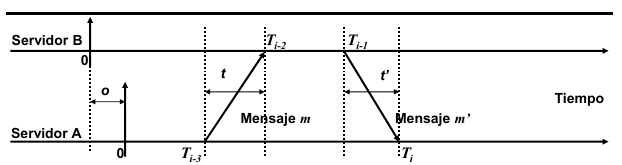
\includegraphics[width=1\textwidth]{img/ntp.png}
  \end{center}

Con la misma nomenclatura de la imagen tenemos:

\begin{align}
T_{i-3}&=430 \\
T_{i-2}&=10050\\
T_{i-1}&= 12270\\
T_{i}&=2995
\end{align}

donde los tiempos los hemos tomado midiendo desde las 16:34:13, para hacer los números más pequeños y manejables (trabajando en milisegundos). \textcolor{green}{Hay una pequeña errata: $T_{i-2}=10480$ porque medimos desde 16:34:13 y para que fuera 10050 tendríamos que estar midiendo desde 16:34:13:430}

Nuestro objetivo es calcular $o$, que es la diferencia de tiempos entre ambos relojes. Observando el esquema, podemos deducir las ecuaciones:
\begin{align}
T_{i-3}+o+t=T_{i-2}\\
T_{i}+o=T_{i-1}+t'
\end{align}
Tampoco conocemos $t$ n $t'$, pues no sabemos el tiempo que ha tardado el mensaje en ser transmitido. Si sumamos las dos ecuaciones y despejamos $o$ de la nueva ecuación nos queda:
\[o=\underbrace{\frac{T_{i-2}+T_{i-1}-T_i-T_{i-3}}{2}}_{o_i}+\frac{t'-t}{2}\]

Así, tenemos $o$ escrito como la suma de un valor conocido más una desviación. Puesto que todos los tiempos son positivos, tenemos que $t+t'>t'-t$ por lo que podemos acotar $o$ mediante:
\[o_i-\frac{\overbrace{t'+t}^{d_i}}{2}\leq o \leq o_i + \frac{\overbrace{t'+t}^{d_i}}{2}\]

Así, podemos decir que la deriva es: $o_i=9447.5ms$ con una precisión de $\pm 172.5 ms\footnote{Para obtener t'+t restamos las dos ecuaciones del sistema}$


  \end{problem}

  \begin{problem}[17]
  Los protocolos de comunicaciones pueden ser orientados a conexión o no
  orientados a conexión. Describir los pros y los contras de cada uno de
  ellos para su utilización como medio de transporte de un sistema distribuido,
  e identificar el tipo más adecuado para realizar accesos a un servidor
  iterativo o a un servidor concurrente.
  \solution
\begin{itemize}
\item \textbf{Orientado a conexión: TCP}

 \subitem \textbf{Ventajas:}
 \begin{itemize}
\item Confiable: se garantiza recepción del mensaje.
\item Garantiza entrega de mensajes en el orden correcto.
\item Incorpora control de flujo.
\item No hay límite en el tamaño de los mensajes.
\end{itemize}
\subitem \textbf{Desventajas:}
\begin{itemize}
\item Mayor sobrecarga de procesamiento (mantener conexión).
\item Mayor información de protocolo en las cabeceras.
\item Limitado a la comunicación 1 a 1.
\end{itemize}

\item \textbf{No orientado a conexión: UDP}
\end{itemize}
 \subitem \textbf{Ventajas:}
 \begin{itemize}
\item Comunicación 1 a N utilizando broadcast y multicast.
\item Menos sobrecarga (no hay que mantener conexión).
\item Menor información de protocolo en las cabeceras.
\end{itemize}
\subitem \textbf{Desventajas:}
\begin{itemize}
\item No hay información sobre mensajes consecutivos.
\item Posible pérdida de mensajes o duplicidad de los mismos.
\item Mensajes de tamaño limitado.
\item No hay control de flujo.
\end{itemize}

Una vez hemos analizado estas ventajas e inconvenientes de ambos protocolos, podemos decidir cuál de ellos es más ventajoso utilizar en cada uno de los casos planteados:

\begin{itemize}
\item \textbf{Servidor Concurrente:}
\begin{itemize}
\item Generalmente utilizan protocolos orientados a conexión.
\item Cuando se recibe una nueva petición de conexión se crea un
nuevo proceso o hilo que se encargará de gestionarla.
\item Ejemplos: servidores web (HTTP), servidores de acceso
remoto (Telnet), servidores FTP.
\item Excepciones: servidor TFTP (usa protocolo UDP)
\end{itemize}
\item \textbf{Servidor Iterativo:}
\begin{itemize}
\item Generalmente utilizan protocolos NO orientados a conexión.
\item Servidores del tipo petición / respuesta que no almacenan
estado.
\item Ejemplos: servidores DNS o servidores DHCP.
\item Excepciones: servidor Daytime (utiliza protocolo TCP).
\end{itemize}
\end{itemize}
  \end{problem}

  \begin{problem}[18]
  Los servidores de un sistema distribuido pueden ser de dos tipos: sin estado
  \textit{(stateless)}, es decir, que no recuerdan la historia de peticiones anteriores realizadas
  por el cliente; o con estado \textit{(statefull)}, en caso contrario. Identificar el tipo de protocolo de transporte más
  adecuado (orientado o no orientado a conexión) para realizar los accesos
  a cada uno de estos tipos de servidores.
  \solution

  Para los servidores \textbf{statefull}, por su facilidad para identificar mensajes consecutivos de un mismo cliente, son
más apropiados los \textbf{protocolos orientados a conexión}. Si se usasen protocolos no orientados a conexión habría que incluir un campo adicional en cada mensaje para asociarlos a un mismo cliente.

No obstante, existen algunas excepciones, como DHCP que utiliza UDP pero guarda un estado asociado a cada cliente (qué dirección IP tiene asignada)

 Los servidores \textbf{stateless} no guardan información alguna asociada a cada cliente. Generalmente son del tipo petición respuesta donde no se guarda información asociada a cada cliente ni importa el orden de los mensajes enviados.

 Un ejemplo son los servidores DNS, servidores web o NTP. Un cliente solicita una
pagina web, sin importar qué páginas web ha solicitado anteriormente. Ya que no hace falta identificar mensajes consecutivos de un mismo cliente son más apropiados los \textbf{protocolos no orientados a conexión} como UDP pues tienen menos sobrecarga.

Como en todo dentro de la informática existen expeciciones como son los servidores web o los servidores web que utilizan TCP, probablemente debido a la limitación en el tamaño del mensaje en
UDP.
  \end{problem}

  \begin{problem}[19]
  Un servicio de autenticación en una red de área local funciona
mediante un mecanismo de comunicación basado en Remote Procedure Calls,
RPCs genéricas. Dispone de las siguientes funciones:
  \begin{itemize}
    \item Autenticación de usuario: Recibe como parámetros un
identificador de usuario y su contraseña, y devuelve un código de
retorno 0 si usuario y contraseña son correctos, y -1 en caso contrario.
    \item Cambio de contraseña: Recibe como parámetros un
identificador de usuario, su contraseña actual y la nueva contraseña que
 se desea registrar. Devuelve un código de retorno 0 si se ha realizado
correctamente la actualización, y -1 en caso contrario.
    \item Obtención de lista de privilegios asociados a un usuario: Recibe como parámetro
    un identificador de usuario. Si dicho usuario existe en el sistema, devuelve
    un código de retorno 0 y dos listas de longitud variable: la primera con
    todos los atributos definidos en el sistema para el usuario, separados
    por espacios; y la segunda con los nombres de todos los servidores de la
    red a los que tiene acceso, también separados por espacios. Si el usuario
    no existe, devuelve un código de retorno -1.
  \end{itemize}
  Los identificadores de usuario, contraseñas, atributos de usuario y nombres
  de servidores son cadenas de caracteres ASCII que tienen un tamaño máximo
  de 16 caracteres.
  \begin{itemize}
    \item Suponiendo que la red es homogénea (el mismo tipo de sistema
para clientes y servidor), proponer una estructura de mensaje de
petición y una estructura de mensaje de respuesta para la comunicación
entre client stub y server stub adecuado a las tres RPCs. (Describir la
estructura en pseudocódigo o en lenguaje C, de modo que quede
suficientemente clara).
    \item Introducir los cambios necesarios en el mensaje de petición
 de la RPC de autenticación de usuario para soportar una red no
homogénea (clientes y servidor de distintos tipos).
    \item Comentar los problemas de seguridad que presenta el diseño
elegido para esta aplicación, y proponer alternativas para resolverlo.
     \end{itemize}
  \solution

  Olakase

  \end{problem}

  \begin{problem}[20]
  Los ordenadores de una empresa están conectados siguiendo el modelo cliente
servidor, de acuerdo con la siguiente organización jerárquica de dominios
administrativos:
\begin{center}
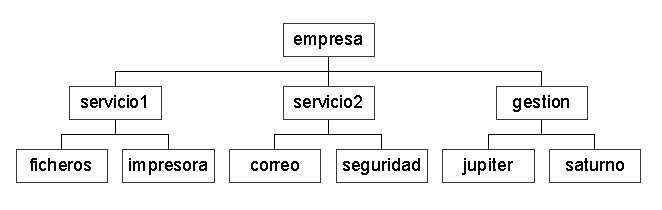
\includegraphics[width=1\textwidth]{img/si2-t4-ej-dom2.png}
\end{center}

   Las hojas del árbol representan ordenadores, los restantes nodos
dominios. Cada dominio tiene un servidor de nombres que reside en un
ordenador, cuyo nombre coincide con el del dominio, con capacidad de
almacenamiento local de resultados de consultas a otros dominios \textit{(cache)}. Se supone que al principio las caches están todas vacías.

    \ppart Escribir los nombres completos en el dominio global de todos los ordenadores
    situados en las hojas del árbol.
    \ppart Detallar los mensajes necesarios para que el ordenador jupiter localice
    el servidor seguridad en el directorio a partir de su nombre en la red.
    \ppart Inmediatamente después de la consulta anterior, el
ordenador saturno desea localizar el servidor seguridad. Indicar el
flujo de mensajes correspondiente.
    \ppart Suponemos que el sistema de nombres utiliza el estándar X500. Decir qué ordenadores contienen un \textit{Directory User Agent} y cuáles contienen un \textit{Directory System Agent}.
    \ppart Escribir tres parejas de ordenadores entre los que se utilice el \textit{Directory Access Protocol}.
    \ppart Escribir tres parejas de ordenadores entre los que se utilice el \textit{Directory System Protocol}.
    \ppart Para cada uno de los cuatro servidores (ficheros,
impresora, correo y seguridad) elegir razonadamente el mecanismo de
transporte aconsejable para conectar a ellos los ordenadores clientes:
peer to peer orientado a conexión, peer to peer no orientado a conexión,
 RPC o MOM.

\solution

\spart
\begin{itemize}
\item ficheros.servicio1.empresa
\item impresora.servicio1.empresa
\item correo.servicio2.empresa
\item seguridad.servicio2.empresa
\item jupiter.gestion.empresa
\item saturno.gestion.empresa
\end{itemize}

\spart
\begin{center}
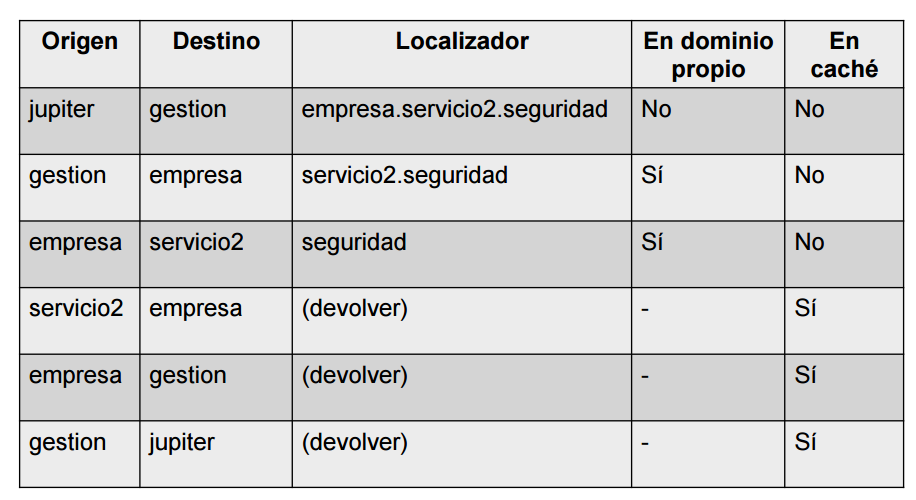
\includegraphics[width=1\textwidth]{img/H2_E20_B.png}
\end{center}

\spart
\begin{center}
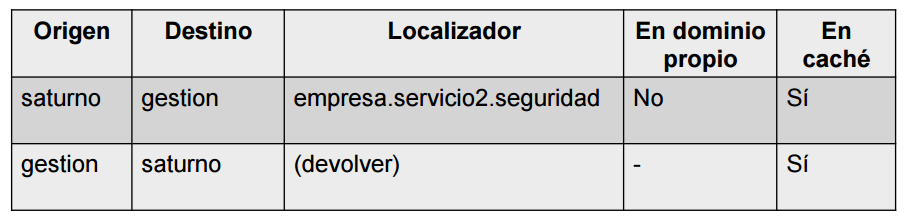
\includegraphics[width=1\textwidth]{img/H2_E20_C.png}
\end{center}

\spart
\begin{itemize}
\item \textbf{Directory User Agent}

ficheros, impresora, correo, seguridad, jupiter, saturno
\item \textbf{Directory System Agent}

empresa, servicio1, servicio2, gestion
\end{itemize}

\spart

\begin{itemize}
\item fichero – servicio1
\item correo – servicio2
\item seguridad – gestion
\end{itemize}

\spart
\begin{itemize}
\item servicio1 – empresa
\item servicio2 – empresa
\item gestion – empresa
\end{itemize}

\spart

\yoP

TO BE CONTINUED...

Me da mucha pereza y no estoy seguro de lo que quieren pero creo que habría que pensar que para la impresora nos interesa cola de mensajes, para el correo igual, para la parte de seguridad posiblemente necesitemos RTP, para la de ficheros TCP si es sólo escritura directa, o incluso UDP y para la parte de gestión pues no sabemos nada porque no tenemos detalles.
\end{problem}
